\documentclass{beamer}

\usepackage{txfonts}
\usepackage{hyperref}
\usepackage{fancybox}
\usepackage{xfrac}
\usepackage{cancel,slashbox}

\newcommand{\heart}{\ensuremath\heartsuit}

\usepackage{mathtools,amssymb}
\newcommand{\myarrow}{\scalebox{2}[2]{$\mathclap{\curvearrowleft}\mkern2.2mu
                                                 \mathclap{\curvearrowright}$}}

\DeclareMathOperator{\Bin}{\mathrm{Bin}}
\DeclareMathOperator{\Max}{\mathrm{Max}}
\DeclareMathOperator{\Cov}{\mathrm{Cov}}
\DeclareMathOperator{\Covr}{\mathrm{Covr}}
\DeclareMathOperator{\Corr}{\mathrm{Corr}}

\hypersetup{colorlinks=false,linkbordercolor=red,linkcolor=green,pdfborderstyle={/S/U/W 1}}

\addtobeamertemplate{navigation symbols}{}{ \hspace{1em}    \usebeamerfont{footline}%
    \insertframenumber / \inserttotalframenumber}

\geometry{papersize={15cm,15cm}}
\usepackage{lipsum}

\makeatletter
\newenvironment<>{contdproof}[1][\proofname]{%
    \par
    \def\insertproofname{#1\@addpunct{.}}%
    \usebeamertemplate{proof begin}#2}
  {\usebeamertemplate{proof end}}
\makeatother


\setbeamertemplate{theorems}[numbered]

\newtheorem{remark}{Remark}



\newtheorem*{nonumdefinition}{Definition}
\newtheorem*{nonumproblem}{Problem}
\newtheorem*{nonumcorollary}{Corollary}
\newtheorem*{nonumlemma}{Lemma}
\newtheorem*{nonumproof}{Proof}
\newtheorem*{nonumtheorem}{Theorem}
\newtheorem*{nonumremark}{Remark}
\newtheorem*{answer}{Answer}
\newtheorem*{nonumremarks}{Remarks}
\newtheorem*{nonumexamples}{Examples}
\newtheorem*{nonumsolution}{Solution}
\newtheorem*{nonumexample}{Example}
\newtheorem*{nonumproposition}{Proposition}
\newtheorem{proposition}[theorem]{Proposition}

\usepackage{tikz}
\newcommand*\mycirc[1]{%
  \tikz[baseline=(C.base)]\node[draw,circle,inner sep=.7pt](C) {#1};\:
}

\newcommand\myheading[1]{%
  \par\bigskip
  {\color{blue}{\large #1}}\par\smallskip}

%\usetheme{Warsaw}
%\usetheme{Berkeley} %sample 1

\usetheme{Berlin} % sample 2
%\usetheme{AnnArbor} % sample 3

\let\otp\titlepage
\renewcommand{\titlepage}{\otp\addtocounter{framenumber}{-1}}

\title{Lecture 16 : Independence, Covariance and Correlation of Discrete Random Variables}
\author{}
\date{}

\begin{document}
\begin{frame}[plain]
\titlepage
\end{frame}

\begin{frame}
\begin{nonumdefinition}
Two discrete random variables $X$ and $Y$ defined on the same sample space are said to be independent if for nay two numbers $x$ and $y$ the two events $(X=x)$ and $(Y=y)$ are independent $\Leftrightarrow$
\begin{equation*}
\text{\includegraphics{figure/fig1.eps}}\tag{*}\label{eq-*}
\end{equation*}
\end{nonumdefinition}
\end{frame}

\begin{frame}
Now \eqref{eq-*} say the \underline{joint} $pmf$ $P_{X,Y}(x,y)$ is determined by the \underline{marginal} $pmf$'s $P_{X}(x)$ and $P_{Y}(y)$ by taking the product.

\begin{nonumproblem}
In case $X$ and $Y$ are independent how do you recover the matrix (table) representing $P_{X,y}(x,y)$ from its margins?
\end{nonumproblem}
\end{frame}

\begin{frame}
Let's examine the table for the standard example
\begin{center}
\renewcommand{\arraystretch}{1.2}
\begin{tabular}{c|c|c|c|c|c}
\backslashbox{$X$}{$Y$} & 0 & 1 & 2 & 3 & \\
\hline
0 & $\frac{1}{8}$ & $\frac{2}{8}$ & $\frac{1}{8}$ & 0 & $\frac{1}{2}$\\
\hline
1 & 0 & $\frac{1}{8}$ & $\frac{2}{8}$ & $\frac{1}{8}$ & $\frac{1}{2}$\\
\hline
 & $\frac{1}{8}$ & $\frac{3}{8}$ & $\frac{3}{8}$ & $\frac{1}{8}$ & 
\end{tabular}
\end{center}

Note that

\smallskip
\qquad $X = \sharp$ of heads on the first toss

\qquad $Y$ = total $\sharp$ of heads in all three tosses
\smallskip

So we wouldn't expect $X$ and $Y$ to be independent (if we know $X=1$ that restricts the values of $Y$.)
\end{frame}

\begin{frame}
Lets use the formula \eqref{eq-*}

It says the following.

Each position inside the table corresponds to two positions on the margins
\begin{enumerate}
\item Go to the right

\item Go Down

\smallskip
\centerline{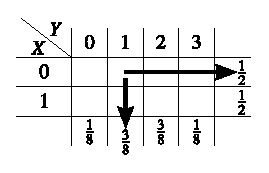
\includegraphics{figure/fig2.eps}}
\smallskip
\end{enumerate}

So in the picture
\begin{enumerate}
\item If we go right we get $\dfrac{1}{2}$

\item If we go down we get $\dfrac{3}{8}$
\end{enumerate}
\end{frame}

\begin{frame}
If $X$ and $Y$ are independent then the formula \eqref{eq-*} says the entry inside the table is obtain by multiplying 1 and 2

\smallskip
\centerline{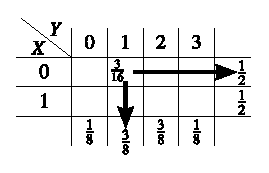
\includegraphics{figure/fig3.eps}}
\smallskip

So if $X$ and $Y$ wave independent then we would set
\begin{equation*}
\renewcommand{\arraystretch}{1.2}
\begin{array}{c|c|c|c|c|c}
\text{\backslashbox{$X$}{$Y$}} & 0 & 1 & 2 & 3 &\\
\hline
0 & \frac{1}{16} & \frac{3}{16} & \frac{3}{16} & \frac{1}{16} & \frac{1}{2}\\
\hline
1 & \frac{1}{16} & \frac{3}{16} & \frac{3}{16} & \frac{1}{16} & \frac{1}{2}\\
\hline
 & \frac{1}{8} & \frac{3}{8} & \frac{3}{8} & \frac{1}{8} & 
\end{array}\tag{$\sharp$}\label{eq-sharp}
\end{equation*}
\end{frame}

\begin{frame}
So as we expected for the basic example \underline{$X$ and $Y$ are not independent.}

From \eqref{addeq-*} on page 5 we have
\begin{equation*}
\renewcommand{\arraystretch}{1.2}
\begin{array}{c|c|c|c|c|}
\text{\backslashbox{$X$}{$Y$}} & 0 & 1 & 2 & 3\\
\hline
0 & \frac{1}{8} & \frac{2}{8} & \frac{1}{8} & 0\\
\hline
1 & 0 & \frac{1}{8} & \frac{2}{8} & \frac{1}{8}\\
\hline
\end{array}\tag{*}\label{addeq-*}
\end{equation*}
This is not the same as \eqref{eq-sharp}.
\end{frame}

\begin{frame}
\myheading{Covariance and Correlation}

In the ``real world'' e.g., the newspaper one often hears (reeds) that two quantities are \underline{correlated}. This word is often taken to be synonymous with \underline{causality}. This is not correct and the difference is extremely important even in reel life. Here are two real word examples of correlations.
\begin{enumerate}
\item Being rich and driving on expensive car.

\item Smoking and lung cancer.
\end{enumerate}
In the first case there is no causality whereas it is critical that in the second there is.
\end{frame}

\begin{frame}
Statisticians can observe correlations (say for 2) but not causalities.

\myheading{Now for the mathematical theorem Covariance}

\begin{nonumdefinition}
Suppose $X$ and $Y$ are discrete and defined on the same sample space. Then the covariance $\Cov(X,Y)$ between $X$ and $Y$ is defined by
\begin{align*}
\Cov (X,Y) &= E((X-\mu_{X})(Y-\mu_{Y}))\\[3pt]
           &= \sum\limits_{x,y}(x-\mu_{X})(y-\mu_{Y})P_{X,Y}(x,y)
\end{align*}
\end{nonumdefinition}
\end{frame}

\begin{frame}
\begin{nonumremark}
$$
\Cov (X,X)=E\left((X-\mu_{X})^{2}\right)=V(X)
$$
There is a \underline{shortcut formula} for covariance.
\end{nonumremark}

\begin{nonumtheorem}[Shortcut formula]
$$
\Cov(X,Y)=E(XY)-\mu_{X}\mu_{Y}
$$
\end{nonumtheorem}

\begin{nonumremark}
If you put $X=Y$ you get the shortcut formula for the variance
$$
V(X)=E(X^{2})-\mu^{2}_{X}
$$
\end{nonumremark}
\end{frame}

\begin{frame}
Recall that $X$ and $Y$ are independent $\Leftrightarrow P_{X,Y}(x,y)=P_{X}(x)P_{Y}(y)$.

\begin{nonumtheorem}
$X$ and $Y$ are independent
$$
\Rightarrow\quad \Cov (X,Y)=0
$$
(the reverse implication does not always hold).
\end{nonumtheorem}

\begin{nonumproof}
$$
E(XY)=\sum\limits_{x,y}xy P_{X,Y}(x,y)
$$
\end{nonumproof}
\end{frame}

\begin{frame}
\begin{proof}[Proof (Cont.)]
Now if $X$ and $Y$ are independent then
$$
P_{X,Y}(x,y)=P_{X}(x)P_{Y}(y)
$$
So 
\begin{align*}
E(XY) &= \sum\limits_{x,y}xy P_{X}(x)P_{Y}(y)\\[3pt]
      &= \sum\limits_{x} \times P_{X}(x)\sum\limits_{y}yP_{y}(y)\\[3pt]
      &= \mu_{X}\mu_{Y}
\end{align*}
Hence
\begin{align*}
\Cov (X,Y) &= \mu_{X}\mu_{Y}-\mu_{X}\mu_{Y}\\[3pt]
           &= 0
\end{align*}
\end{proof}
\end{frame}

\begin{frame}
\myheading{Corelation}

Let $X$ and $Y$ be as before and suppose $\sigma_{X}=\sqrt{V(X)}$ and $\sigma_{Y}=\sqrt{V(Y)}$ be their respective standard deviations.

\begin{nonumdefinition}
The correlation, $\Corr (X,Y)$ or $\rho_{X,Y}$ or just $\rho$, is defined by
$$
\rho_{X,Y}=\dfrac{\Cov(X,Y)}{\sigma_{X}\sigma_{Y}}
$$
\end{nonumdefinition}
\end{frame}

\begin{frame}
\begin{nonumproposition}
$$
-1\leq \rho_{X,Y}\leq 1
$$
\end{nonumproposition}

\begin{nonumtheorem}
The meaning of correlation.
\begin{enumerate}
\item $e_{X,Y}=1\Leftrightarrow Y=aX+b$ with $a>0$ ``perfectly correlated''

\item $P_{X,Y}=-1\Leftrightarrow Y=aX+b$ with $a<0$ ``perfectly anticorrelated''

\item $X$ and $Y$ are independent $\Rightarrow \rho_{X,Y}=0$ but not conversely as we will see Pg. 18-21.
\end{enumerate}
\end{nonumtheorem}
\end{frame}

\begin{frame}
\myheading{A Good Citizen's Problem}

Suppose $X$ and $Y$ are discrete with joint $pmf$ given by that of the basic example \eqref{addeq-*}
\begin{center}
\renewcommand{\arraystretch}{1.2}
\begin{tabular}{c|c|c|c|c|}
\backslashbox{$X$}{$Y$} & 0 & 1 & 2 & 3\\
\hline
0 & $\frac{1}{8}$ & $\frac{2}{8}$ & $\frac{1}{8}$ & 0\\
\hline
1 & 0 & $\frac{1}{8}$ & $\frac{2}{8}$ & $\frac{1}{8}$\\
\hline
\end{tabular}
\end{center}
\begin{itemize}
\item[(i)] Compute $\Cov (X,Y)$

\item[(ii)] Compute $\rho_{X,Y}$
\end{itemize}

\begin{nonumsolution}
We first need the marginal distributions.
\end{nonumsolution}
\end{frame}

\begin{frame}
\begin{nonumsolution}[Cont.]
\begin{center}
\begin{tabular}{c|c|c|}
$X$ & 0 & 1\\
\hline
$P(X=x)$ & $\frac{1}{2}$ & $\frac{1}{2}$\\
\hline
\end{tabular}
\end{center}
So $X\sim \Bin \left(1,\dfrac{1}{2}\right)$ so $E(X)=\dfrac{1}{2}$, $V(X)=\dfrac{1}{4}$ and $\sigma_{X}=\dfrac{1}{2}$
\begin{center}
\renewcommand{\arraystretch}{1.2}
\begin{tabular}{c|c|c|c|c|}
$Y$ & 0 & 1 & 2 & 3 \\
\hline
$P(Y=y)$ & $\frac{1}{8}$ & $\frac{3}{8}$ & $\frac{3}{8}$ & $\frac{1}{8}$\\
\hline
\end{tabular}
\end{center}
So $Y\sim \Bin \left(3,\dfrac{1}{2}\right)$ so $E(Y)=\dfrac{3}{2}$, $V(X)=\dfrac{3}{4}$ so $\sigma_{Y}=\dfrac{\sqrt{3}}{2}$.

\underline{Now we need $E(XY)$} (the hard part)
$$
E(XY)=\sum\limits_{xy}xy \ P(X=x,Y=y)
$$
Trick - We are summing over entries in the matrix times $xy$ so potentially \underline{eight} terms.
\end{nonumsolution}
\end{frame}

\begin{frame}
\begin{nonumsolution}[Cont.]
But the four terms from first row don't contribute because $x=0$ so $xy=0$. Also the first term in the second row doesn't  contribute since $y=0$. So there are only \underline{three} terms.
\begin{align*}
E(XY) &= (1)(1)\left(\dfrac{1}{8}\right)+(1)(2)\left(\dfrac{2}{8}\right)+(1)(3)\left(\dfrac{1}{8}\right)\\
      &= \frac{1}{8}[1+4+3]=\frac{8}{8}=1
\end{align*}
So
\begin{align*}
\Cov (X,Y) &= E(XY)-\mu_{X}\mu_{Y}\\[3pt]
           &= 1-\left(\frac{1}{2}\right)\left(\dfrac{3}{2}\right)=\frac{1}{4}
\end{align*}
\end{nonumsolution}
\end{frame}

\begin{frame}
\begin{nonumsolution}[Cont.]
\begin{itemize}
\item[(ii)] 
\begin{tabbing}
$\rho_{X,Y}$ \== $\dfrac{\Cov(X,Y)}{\sigma_{X}\sigma_{Y}}$\\[5pt]
            \>= $\dfrac{\sfrac{1}{4}}{\left(\frac{1}{2}\right)\left(\frac{\sqrt{3}}{2}\right)}=\dfrac{\sfrac{1}{\cancel{4}}}{\sfrac{\sqrt{3}}{\cancel{4}}}$\\[5pt]
            \>= $\dfrac{-1}{\sqrt{3}}=\dfrac{\sqrt{3}}{3}$
\end{tabbing}
\end{itemize}
\end{nonumsolution}
\end{frame}

\begin{frame}
\myheading{A cool counter example}

We need an example to show
$$
\Cov (X,Y)=0 \not\Rightarrow X \text{~ and~ } Y \text{ are independent}
$$
So we need to describe a $pmf$. Here is its ``graph''
\begin{equation*}
\begin{array}{c}
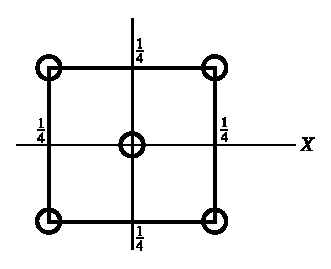
\includegraphics{figure/fig4.eps}\tag{$\sharp$}
\end{array}\label{addeq-sharp}
\end{equation*}
What does this mean.

The corner points (with the zeroes) are $(1,1)$, $(1,-1)$, $(-1,-1)$ and  $(-1,1)$ (clockwise)
\end{frame}

\begin{frame}
and of course the origin.

Here is the bar graph

\smallskip
\centerline{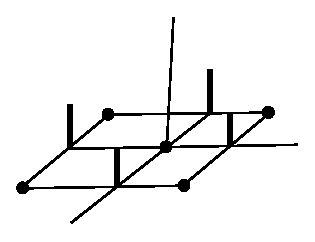
\includegraphics{figure/fig5.eps}}
\smallskip

The vertical spikes have height $\sfrac{1}{4}$.

The matrix of the $pmf$ is
\begin{equation*}
\begin{array}{c|c|c|c|c}
\text{\backslashbox{$X$}{$Y$}} & -1 & 0 & 1 & \\
\hline
-1 & 0 & \frac{1}{4} & 0 & \frac{1}{4}\\
\hline
0 & \frac{1}{4} & 0 & \frac{1}{4} & \frac{1}{2}\\
\hline
1 & 0 & \frac{1}{4} & 0 & \frac{1}{4}\\
  & \frac{1}{4} & \frac{1}{2} & \frac{1}{4} &
\end{array}\tag{*}\label{addeq1-*}
\end{equation*}
I have given the marginal distributions.
\end{frame}

\begin{frame}
Here are the tables for the marginal distributions
\begin{align*}
& \begin{array}{|c|c|c|c|}
    X & -1 & 0 & 1\\
\hline
    P(X=x) & \frac{1}{4} & \frac{1}{2} & \frac{1}{4}\\
\hline
  \end{array}\qquad\quad E(X)=0\\[10pt]
& \begin{array}{|c|c|c|c|}
Y & -1 & 0 & 1\\
\hline
P(Y=y) & \frac{1}{4} & \frac{1}{2} & \frac{1}{4}\\
\hline
  \end{array}\qquad\quad E(Y)=0
\end{align*}
Now for the covariance.

Here is the really cool thing.

\underline{Every term} in the Formula for $E(XY)$ so $E(XY)$ is the sum of nine zeroes so $E(XY)=0$.

So
$$
\Cov (X,Y)=E(XY)-E(X)E(Y)=0-(0)(0)
$$
\end{frame}

\begin{frame}
But $X$ and $Y$ are not independent because if we go from the outside in we get
\begin{equation*}
\begin{array}{c|c|c|c|c}
\text{\backslashbox{$X$}{$Y$}} & -1 & 0 & 1 & \\
\hline
-1 & \sfrac{1}{16} & \sfrac{1}{8} & \sfrac{1}{16} & \sfrac{1}{4}\\
\hline
0 & \sfrac{1}{8} & \sfrac{1}{4} & \sfrac{1}{8} & \sfrac{1}{2}\\
\hline
1 & \sfrac{1}{16} & \sfrac{1}{8} & \sfrac{1}{16} & \sfrac{1}{4}\\
\hline
  & \sfrac{1}{4} & \sfrac{1}{2} & \sfrac{1}{4} & 
\end{array}\tag{**}\label{eq-**}
\end{equation*}
\eqref{addeq1-*} $\neq$ \eqref{eq-**}.

So $X$ and $Y$ are not independent.
\end{frame}

\begin{frame}
It turns out the picture \eqref{addeq-sharp} gives us another counter example. Consider the following three events

\smallskip
\centerline{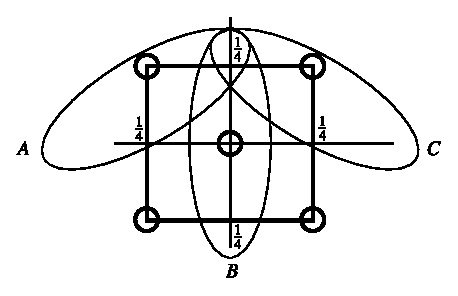
\includegraphics{figure/fig6.eps}}
\smallskip
\begin{align*}
\text{So~ } A &= \{(0,1), (-1,1), (-1,0)\}\\[3pt]
            B &= \{(0,1), (0,0), (0,-1)\}\\[3pt]
            C &= \{(0,1), (1,1), (1,0)\}
\end{align*}
\end{frame}

\begin{frame}
We claim
\begin{enumerate}
\item $A$, $B$, $C$ are pairwise independent but not independent.

That is
\begin{align*}
P(A\cap B) &= P(A)P(B)\\
P(A\cap C) &= P(A)P(C)\\
P(B\cap C) &= P(B)P(C)
\end{align*}
but 
$$
P(A\cap B\cap C)=P(A)P(B)P(C)
$$
\end{enumerate}
\end{frame}

\begin{frame}
Let's check this
\begin{align*}
P(A) &= P(\{(0,1),(-1,1),(-1,0)\}\\
     &=\frac{1}{2}\\
P(B) &= P(\{(0,1),(0,0),(0,-1)\}\\
     &= \frac{1}{2}\\
P(C) &= P(\{(0,1),(1,1),(1,0)\}\\
     &= \frac{1}{2}\\
A\cap B &= \{(0,1)\}\\
A\cap C &= \{(0,1)\}\\
B\cap C &=\{(0,1)\}
\end{align*}
So they all of probability $\dfrac{1}{4}$.
\end{frame}

\begin{frame}
\centerline{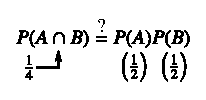
\includegraphics{figure/fig7.eps}}

yes and the some for $A\cap C$ and $B\cap C$.

But $A\cap B\cap C=\{(0,1)\}$

So
$$
P(A\cap B\cap C)=P((0,1))=\frac{1}{4}
$$
But
\begin{align*}
P(A)P(B)P(C) &= \left(\frac{1}{2}\right)\left(\frac{1}{2}\right)\left(\frac{1}{2}\right)\\
             &= \frac{1}{8}
\end{align*}
So
$$
P(A\cap B\cap C)\neq P(A)P(B)P(C)
$$
\end{frame}

\begin{frame}
\myheading{An Analogy with Vectors}

Here is how I remember the properties of covariance (I learned statistics long after I learned about vectors). This analogy really comes from advanced mathematics on the notion of a ``Hilbert space''. 

\smallskip
\centerline{\includegraphics{figure/fig8.eps}}
\smallskip

So
$$
V(X)=\Cov(X,X)\longleftrightarrow \overrightarrow{u}-\overrightarrow{u}=||\,\overrightarrow{u}\,||^{2}
$$
\end{frame}

\begin{frame}
So

\smallskip
\centerline{\includegraphics{figure/fig9.eps}}
\smallskip

Now gives two vectors in the plane the (un oriented) angle between them which I will denote $\nless (\overrightarrow{u},\overrightarrow{v}$ is the inverse cosine of $\dfrac{\overrightarrow{u}\cdot \overrightarrow{v}}{||\,\overrightarrow{u}\,||~||\,\overrightarrow{v}\,||}$ that is
$$
\cos (\nless (\overrightarrow{u},\overrightarrow{v}))=\dfrac{\overrightarrow{u}\cdot \overrightarrow{v}}{||\,\overrightarrow{u}\,||~||\,\overrightarrow{v}\,||}
$$

\smallskip
\centerline{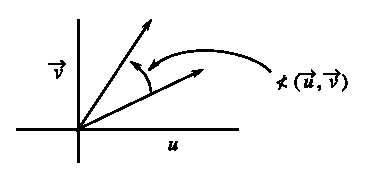
\includegraphics{figure/fig10.eps}}
\end{frame}

\begin{frame}
So what does this correspond to in the world of random variables

\smallskip
\centerline{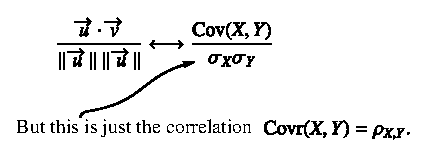
\includegraphics{figure/fig11.eps}}
$$
\rho_{X,Y}\longrightarrow \text{Cos}\nless (\overrightarrow{u}, \overrightarrow{v})
$$

So what do we get from all this?
\end{frame}

\begin{frame}
\myheading{Positive Correlation}
$$
\cos \nless (\overrightarrow{u},\overrightarrow{v})=1\Longleftrightarrow \nless (\overrightarrow{u}, \overrightarrow{v})=0
$$
\centerline{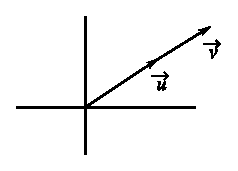
\includegraphics{figure/fig12.eps}}
\smallskip

$\overrightarrow{u}$ and $\overrightarrow{v}$ lie in the same ray (half-line) so $\overrightarrow{u}=a\overrightarrow{v}$, $a>0$.

Now what about correlation
$$
\text{Corr}(X,Y)=1\Longleftrightarrow Y=aX+b\text{~~ with~~ } a>0.
$$

\myheading{Negative Correlation}

\centerline{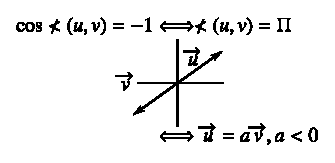
\includegraphics{figure/fig13.eps}}
\end{frame}

\begin{frame}
What about correlation
$$
\Corr (X,Y)=-1\Longleftrightarrow Y=aX+b\text{~ with~ } a<0
$$

\myheading{Zero Correlation}
\begin{align*}
\cos \nless (\overrightarrow{u},\overrightarrow{v}) = 0 &\Longleftrightarrow \overrightarrow{u}\cdot \overrightarrow{v}=0\\
&\Longleftrightarrow \overline{u}\text{~~ and~~ }\overrightarrow{v}\text{~ are orthogonal.}
\end{align*}
\centerline{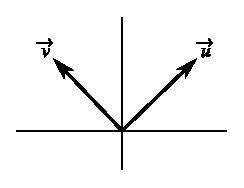
\includegraphics{figure/fig14.eps}}
$$
\Corr(X,Y)=0\Longleftarrow X\text{~~ and~~ } Y \text{~ are independent}
$$
\end{frame}

\begin{frame}
\myheading{Bottom Line}

Intuitively $\rho_{X,Y}$ corresponds to the cosine of the angle between the two random variables $X$ and $Y$.
\end{frame}

\end{document}


